% Cita textual seccion Desarrolo:

% Deben explicarse los metodos numericos que utilizaron
% y su aplicacion al problema concreto involucrado en el trabajo practico.
% Se deben mencionar los pasos que siguieron para implementar
% los algoritmos, las dificultades que fueron encontrando y la
% descripcion de como las fueron resolviendo.

% Explicar tambien como fueron planteadas y realizadas las
% mediciones experimentales. Los ensayos fallidos, hipotesis y
% conjeturas equivocadas, experimentos y metodos malogrados deben
% figurar en esta seccion,
% con una breve explicacion de los motivos de estas fallas
% (en caso de ser conocidas).

\section{Cálculo de normales}

En esta sección resolveremos el problema de calcular los vectores normales a la superficie, conociendo los vectores luz y los valores de la intensidad para cada píxel dado. Resolveremos utilizando el algoritmo de eliminación gaussiana, y veremos en la siguiente sección una forma de optimizar los cálculos aprovechándonos de las propiedades de nuestro problema.

\subsection{Eliminación Gaussiana}

Para cada píxel, tenemos un sistema listo para resolver:

% Sistema de matrices original
\[
\begin{pmatrix}
    s_{x}^{1} & s_{y}^{1} & s_{z}^{1} \\
    s_{x}^{2} & s_{y}^{2} & s_{z}^{2} \\
    s_{x}^{3} & s_{y}^{3} & s_{z}^{3}
\end{pmatrix}
\begin{pmatrix}
    m_{x} \\
    m_{y} \\
    m_{z}
\end{pmatrix}
=
\begin{pmatrix}
    I_{1} \\
    I_{2} \\
    I_{3}
\end{pmatrix}
\]

Donde los $s_{c}^{i}$ es la coordenada $c$ del vector de luz en la imagen $i$, los $I_i$ las intensidades de luz (del píxel actual) en la imagen $i$, y los $m_j$ nuestras incógnitas. El vector $m = (m_x, m_y, m_z)$ no es exactamente el valor de la normal $n$, sino que $m = I_0 \rho . n$, con $I_0, \rho \in \mathbb{R}$ constantes desconocidas que dependen del objeto. Lo que nos interesa es encontrar el valor de $n$, pero para esto primero debemos hallar $m$. \\

La pregunta ahora es ¿cómo lo resolvemos?. Dado que en principio no sabemos cómo, nos gustaría llevarlo a una forma equivalente que sea mas fácil de resolver. Podemos hacer esta conversión a un sistema equivalente usando el algoritmo de eliminación de Gauss. Lo que hace este algoritmo es llevar una matriz a su forma triangular superior, de dónde luego es muy sencillo hacer los despejes finales. \\

El pseudocódigo del algoritmo de Gauss es el siguiente:

\begin{algorithm}[H]
\begin{algorithmic}
\Function{EliminacionGaussiana}{Matriz M[$n$][$m$]}

    \For{$k \in [1..min(n,m)]$ }
        \For{$i \in [k+1..m]$ }

            \If{M[$k$][$k$] $\neq 0$}
                \State $mult \gets $M[$i$][$k$] $/$ M[$k$][$k$]
                \For{$j \in [k+1..n]$}

                    \State M[$i$][$j$] $\gets$ M[$i$][$j$] - mult*M[$k$][$j$]

                \EndFor
            \Else
                \State Hay un cero en la diagonal!
            \EndIf
        \EndFor
    \EndFor

\EndFunction
\end{algorithmic}
\end{algorithm}

Como puede verse, funciona correctamente solo \textbf{suponiendo que no hay ceros en la diagonal}. Es claro que puede modificarse para que realice intercambios de filas y no tenga el problema del cero, pero veremos que para nuestro problema no es importante. En nuestra implementación aplicaremos el algoritmo de Gauss en la siguiente matriz ampliada:

% Matriz ampliada
\[
\begin{pmatrix}[ccc|c]
    s_{x}^{1} & s_{y}^{1} & s_{z}^{1} & I_{1} \\
    s_{x}^{2} & s_{y}^{2} & s_{z}^{2} & I_{2} \\
    s_{x}^{3} & s_{y}^{3} & s_{z}^{3} & I_{3}
\end{pmatrix}
\]

Para empezar, nuestros $s_{j}^{i}$ incialmente son todos distintos de cero, asi que nunca habrá un cero en la primer fila. Dado que son solo 12 vectores de luces, tomamos todas las posibles combinaciones de tres luces y corrimos el algoritmo de gauss sin pivoteos. En ningun caso se realizó división por cero ni tampoco apareció ningún cero en la diagonal. (El código de lo realizado puede encontrarse en \textit{TestTieneLU.cpp}). Esto cobrará importancia cuando querramos encontrar factorización LU. \\

Dado que pudimos triangular correctamente la matriz ampliada, entonces ya estamos en condiciones de despejar de nuestra matriz de 3 x 4:

\[
\begin{pmatrix}[ccc|c]
    a_{1,1}   & a_{1,2} & a_{1,3} & a_{1, 4} \\
    0         & a_{2,2} & a_{2,3} & a_{2, 4} \\
    0         & 0       & a_{3,3} & a_{3, 4}
\end{pmatrix}
\]

\begin{algorithm}[H]
\begin{algorithmic}

\Function{Despejar}{Matriz M[$n$][$m$]}

    // En X se guardan los m-1 coeficientes solución (Recordemos que M es ampliada)
    \State X[$m-1$] $\gets \{\}$ \\

    \For{$j \in [1..m-1]$ }  (j es indice de columna)

        \If{M[$j$][$j$] $\neq 0$}

            \State X[$j$] $\gets$ M[$j$][$m$] / M[$j$][$j$]

            \For{$i \in [j-1 .. 0]$ }  (i es indice de fila)

                \State M[$i$][$m$] $\gets$ M[$i$][$m$] - ( M[$i$][$j$] * X[$j$] )

            \EndFor

        \Else
            \State Hay un cero en la diagonal!
        \EndIf
    \EndFor

    \State Retornar X

\EndFunction
\end{algorithmic}
\end{algorithm}

Resolviendo el sistema con la forma expuesta, obtenemos el vector solución $m$. Pero $m$ no es lo que buscábamos, sino que queremos obtener el valor de $n$. Recordemos:

\begin{center}
$m = I_0 \rho . (n_x, n_y, n_z) = I_0 \rho . n$
\end{center}

Con $I_0 \rho \in \mathbb{R}$. Tomando norma:

\begin{center}
$\norm{m} = \abs{I_0 \rho} \norm{n}$
\end{center}

Pero $\norm{n} = 1$, pues queremos el vector unitario. Entonces:

\begin{center}
$\norm{m} = \abs{I_0 \rho}$
\end{center}

Sabiendo esto, podemos despejar y obtener el valor de $n$ (con $m \neq 0$):

\begin{center}
$n = \frac{m}{\norm{m}}$
\end{center}

Obtuvimos así para cada píxel vector normal a la superficie.

\subsection{Factorización LU}

Recordemos nuestro sistema para hallar las normales:
\[
\begin{pmatrix}
    s_{x}^{1} & s_{y}^{1} & s_{z}^{1} \\
    s_{x}^{2} & s_{y}^{2} & s_{z}^{2} \\
    s_{x}^{3} & s_{y}^{3} & s_{z}^{3}
\end{pmatrix}
\begin{pmatrix}
    m_{x} \\
    m_{y} \\
    m_{z}
\end{pmatrix}
=
\begin{pmatrix}
    I_{1} \\
    I_{2} \\
    I_{3}
\end{pmatrix}
\]

Una vez fijas las luces a utilizar (en este caso 1,2 y 3) para despejar la normal en cada píxel, debemos resolver el sistema en cada píxel. Es decir, estaremos traingulando una y otra vez una matriz dónde lo único que cambia es el término a la derecha de la igualdad. Por lo tanto, es interesante plantearse si existe una forma de evitar aplicar Gauss en cada punto. \\

La factorización LU podría no existir, pero veámos de que se trata. Dada una matriz $A$, la factorización LU consiste en encontrar dos matrices: una matriz $L$ triangular inferior con unos en la diagonal y una matriz $U$ triangular superior, de forma que se cumpla

\begin{center}
$A$ = $L$.$U$
\end{center}

% Quiza explicar mejor esto
Por lo visto en clase, puede demostrarse que la $L$ tiene en la diagonal unos, ceros por arriba, y por debajo los multiplicadores que se utilizaron en la eliminación Gaussiana para colocar un cero en la triangulación. En la $U$ se colocan ceros debajo de la diagonal y en el resto los coeficientes que quedaron en la matriz ya triangulada. \\

Digamos entonces que ya conocemos la factorización LU para una matriz dada, ¿Cómo la utilizamos para resolver nuestro sistema?

\begin{center}
    $Ax = b$ $\iff$ $LUx = b$
\end{center}

Si consideramos $Ux = y$, nos queda para resolver:

\begin{center}
    $Ly = b$
\end{center}

Donde $L$ es triangular inferior. Por lo tanto podemos despejar y obtener $y$ sin necesidad de aplicar eliminación Gaussiana. Una vez que conocemos $y$, como $U$ también esta triangulada despejamos en:

\begin{center}
    $Ux = y$
\end{center}

Obteniendo así el $x$ que queríamos encontrar inicialmente. \\

Por lo expuesto en la sección anterior, experimentalmente comprobamos que en nuestra matriz de luces podemos aplicar Gauss normalmente sin encontrarnos con ceros en la diagonal y sin tener que hacer ninguna permutación de filas. \\

Por lo visto en la clase teórica, si podemos triangular una matriz usando Gauss sin tener que permutar filas, es suficiente para afirmar que la factorización LU existe, entonces con el procedimiento explicado podemos hallar la descomposicion de nuestra matriz de luces y resolver el sistema mas eficientemente. \\

\newpage
\section{Estimacion de profundidades}

Utilizando los métodos anteriores pudimos resolver el sistema que incluye las luces y calcular las normales para todo píxel de la imagen. Recordemos que para un cierto píxel $(a, b)$ la normal en ese punto es de la forma:

\begin{center}
$n^{(a,b)} = (n_{x}^{a,b}, n_{y}^{a,b}, n_{z}^{a,b})$
\end{center}

A partir de aquí en ocasiones omitiremos el supraíndice $(a,b)$ para relajar la notación cuando es claro cuál es el píxel del que hablamos. Siguiendo con la técnica de fotometría estéreo, el siguiente paso a realizar es el cálculo de las profundidades utilizando estas normales. Para esto, consideramos una aproximación al plano tangente de cada píxel. La ecuaciones que tenemos que resolver son las siguientes, para cada píxel $(x ,y)$.

\begin{center}
\[
    \begin{dcases}
        n_{y} +  n_{z} * (z_{x, y+1} - z_{x, y}) = 0 \\
        n_{x} +  n_{z} * (z_{x+1, y} - z_{x, y}) = 0
    \end{dcases}
\]
\end{center}
O equivalentemente
\begin{center}
\[\begin{dcases}
        n_{z} * z_{x, y+1} - n_{z} *  z_{x, y} = n_{y}  \\
        n_{z} * z_{x+1, y} - n_{z} *  z_{x, y} = n_{x}
    \end{dcases}
\]
\end{center}

Consideremos como sería el sistema matricial para una imagen de 2x3 pixeles, y veremos como puede generalizarse: \\

% \dots \ddots \vdots

\[
\underbrace{
\begin{pmatrix}
    % - n_{z}^{1,1}  &  0                      & 0  & n_{z}^{1,1}    & 0 & 0 & 0 & 0 & 0 \\
    % - n_{z}^{1,1}  &  n_{z}^{1,1}  &  0  & 0 & 0  &  0               & 0 & 0 & 0 & \\
    % 0 & - n_{z}^{1,2}  &  0                   & 0 &  n_{z}^{1,2}   & 0 & 0 & 0 & 0     \\
    % 0 & - n_{z}^{1,2}  &  n_{z}^{1,2}   & 0 &  0  &  0  &  0         & 0 & 0     \\
    % 0 & 0 & - n_{z}^{1,3}  &  0             & 0   &  n_{z}^{1,3}   & 0 & 0 & 0  \\
    % % 0 & 0 & - n_{z}^{1,3}  &  n_{z}^{1,3} & 0 &  0  &  0  &  0  & 0       \\
    % 0 & 0 &  0  &  0 & 0 &  0  &  0  &  0  & 0       \\
    % 0 & 0 & 0 & - n_{z}^{2,1}  &  0         & 0     &  n_{z}^{2,1} & 0 & 0      \\
    % 0 & 0 & 0 & - n_{z}^{2,1}  &  n_{z}^{2,1} & 0 &  0  &  0  &  0      \\
    % 0 & 0 & 0 & 0 & - n_{z}^{2,2}  & 0       & 0  &  n_{z}^{2,2} & 0            \\
    % 0 & 0 & 0 & 0 & - n_{z}^{2,2}  &  n_{z}^{2,2} & 0 &  0  &  0         \\
    % 0 & 0 & 0 & 0 & 0 & - n_{z}^{2,3}  &  0      & 0     &  n_{z}^{2,3}         \\
    % 0 & 0 & 0 & 0 & 0 & 0  &  0      & 0     &  0         \\
    % % 0 & 0 & 0 & 0 & 0 & - n_{z}^{2,3}  &  n_{z}^{2,3} & 0 &  0        \\
    - n_{z}^{1,1}  &  0                      & 0  & n_{z}^{1,1}    & 0 & 0 \\[3pt]
    - n_{z}^{1,1}  &  n_{z}^{1,1}  &  0  & 0 & 0  &  0               \\[3pt]
    0 & - n_{z}^{1,2}  &  0                   & 0 &  n_{z}^{1,2}   & 0     \\[3pt]
    0 & - n_{z}^{1,2}  &  n_{z}^{1,2}   & 0 &  0  &  0      \\[3pt]
    0 & 0 & - n_{z}^{1,3}  &  0             & 0   &  n_{z}^{1,3}  \\[3pt]
    0 & 0 & - n_{z}^{1,3}  &  0 & 0 &  0       \\[3pt]
    % 0 & 0 &  0  &  0 & 0 &  0         \\[3pt]
    0 & 0 & 0 & - n_{z}^{2,1}  &  0         & 0          \\[3pt]
    0 & 0 & 0 & - n_{z}^{2,1}  &  n_{z}^{2,1} & 0       \\[3pt]
    0 & 0 & 0 & 0 & - n_{z}^{2,2}  & 0                  \\[3pt]
    0 & 0 & 0 & 0 & - n_{z}^{2,2}  &  n_{z}^{2,2}         \\[3pt]
    0 & 0 & 0 & 0 & 0 & - n_{z}^{2,3}          \\[3pt]
    0 & 0 & 0 & 0 & 0 & - n_{z}^{2,3}         \\[3pt]
    % 0 & 0 & 0 & 0 & 0 & - n_{z}^{2,3}  &  n_{z}^{2,3} & 0 &  0        \\[3pt]
\end{pmatrix}}_{\text{\Large{M}}}
\underbrace{\begin{pmatrix}
    z_{1, 1} \\[3pt]
    z_{1, 2} \\[3pt]
    z_{1, 3} \\[3pt]
    z_{2, 1} \\[3pt]
    z_{2, 2} \\[3pt]
    z_{2, 3}
\end{pmatrix}}_{\text{\Large{z}}}
=
\underbrace{\begin{pmatrix}
    n_{y}^{1, 1} \\[3pt]
    n_{x}^{1, 1} \\[3pt]
    n_{y}^{1, 2} \\[3pt]
    n_{x}^{1, 2} \\[3pt]
    n_{y}^{1, 3} \\[3pt]
    n_{x}^{1, 3} \\[3pt]
    n_{x}^{2, 1} \\[3pt]
    n_{y}^{2, 1} \\[3pt]
    n_{x}^{2, 2} \\[3pt]
    n_{y}^{2, 2} \\[3pt]
    n_{x}^{2, 3} \\[3pt]
    n_{y}^{2, 3}
\end{pmatrix}}_{\text{\Large{v}}}
\]

\newpage
A modo de ejemplo, tomemos la tercer fila y hagamos el producto:

\begin{center}
    $-n_{z}^{1, 2} * z_{1,2} + n_{z}^{1, 2} * z_{1, 3} \iff n_{z}^{1, 2} * z_{1, 3} -n_{z}^{1, 2} * z_{1,2}$
\end{center}

y vemos que se corresponde con nuestro sistema original. Puede verse además que las dimensiones para realizar el producto cuadran perfectamente. Si $n'$ y $m'$ eran el alto y ancho de la imagen original, la nueva matriz tiene $2*n'*m'$ filas y $n'*m'$ columnas.

Si bien la matriz esta planteada con unas dimensiones en particular, por su forma es sencillo de generalizar. Dado un cierto píxel $(x, y)$, las dos ecuaciones correspondientes son:

\[
\begin{pmatrix}
    0 & \dots & 0 & n_{z} & 0     & \dots &       & n_{z} & \dots  \\
    0 & \dots & 0 & n_{z} & n_{z} & 0     & \dots & \dots & \dots
\end{pmatrix}
\]

Para cada píxel tenemos la primer ecuacion correspondiente a $n_y$, donde los dos $n_z$ están separados a $m'$ de distancia (\textit{ancho de la imagen original}), y en la segunda ecuación se encuentra la correspondiente a $n_x$ donde los dos $n_z$ se encuentran juntos. También puede verse que cada vez que pasamos al siguiente píxel bajando de fila se produce un corrimiento en una columna hacia la derecha. Hay que tener especial cuidado con los bordes de la imagen, porque el producto dará como resultado una ecuación erronea. Para que esto no sea un problema, colocamos ceros en los lugares problemáticos. \\

Queremos entonces resolver el sistema:

\begin{center}
$M z = v$
\end{center}

Multiplicando por $M^{t}$ a ambos lados se obtiene:
\begin{center}
\[\underbrace{M^{t} M}_{\text{A}} z = \underbrace{M^{t} v}_{\text{b}}\]
\end{center}

Para así llegar al sistema final que nos interesa resolver
\begin{center}
$A z = b$
\end{center}

La matriz $A$ no es cualquier cosa, sino que tiene una forma particular. En primer lugar, es simétrica porque es el resultado de haber multiplicado una matriz con su traspuesta.

En este caso si $(a, b)$ es nuestro píxel escribiremos  $n_{a,b}$ en vez de $n^{a,b}$ para no confundir con el exponente que está potenciando al elemento. Veamos como es la forma de $A$, obtenida simplemente haciendo la cuenta $M^t M$


\setul{5pt}{2pt}
\[
\begin{pmatrix}
    \text{\setulcolor{blue} \ul{$2 n_{1,1}^{2}$}}  &  \text{\setulcolor{blue} \ul{$ -n_{1,1}^{2} $}}   &  0        & \text{\setulcolor{blue} \ul{$-n_{1,1}^{2} $}}   & 0         & 0            \\[10pt]

    \text{\setulcolor{blue} \ul{$-n_{1,1}^{2}$}} &  \text{\setulcolor{blue} \ul{$n_{1,1}^{2}$}} +                                \text{\setulcolor{red} \ul{$2 n_{1,2}^{2}$}}   &  \text{\setulcolor{red} \ul{$-n_{1,2}^{2}$}}        & 0     & \text{\setulcolor{red} \ul{$-n_{1,2}^{2}$}}         & 0            \\[10pt]

    0          &  \text{\setulcolor{red} \ul{$-n_{1,2}^{2}$}}  &  \text{\setulcolor{red} \ul{$n_{1,2}^{2}$}} + 2 n_{1,3}^{2} &   0   & 0  & -n_{1,3}^{2}            \\[10pt]

    \text{\setulcolor{blue} \ul{$-n_{1,1}^{2}$}} &  0            &  0           & \text{\setulcolor{blue} \ul{$n_{1,1}^{2}$}} + 2 n_{2,1}^{2} & -n_{2,1}^{2}    & 0            \\[10pt]

    0          &   \text{\setulcolor{red} \ul{$-n_{1,2}^{2}$}} & 0           & -n_{2,1}^{2}                & \text{\setulcolor{red} \ul{$n_{1,2}^{2}$}} + n_{2,1}^{2} + 2 n_{2,2}^{2}    &      -n_{2,2}^{2}  \\[10pt]

    0          &              0&  -n_{1,3}^{2} & 0                          & - n_{2,2}^{2} & n_{1,3}^{2} + n_{2,2}^{2} + 2 n_{2,3}^{2}             \\[10pt]

\end{pmatrix}
\]

Es fácil darse cuenta del patrón. Vamos tomando $p$ el pixel actual, pensando en los píxeles ordenados ($(1,1), (1,2), (1,3), .. $) Colocamos $2p^2$ en la diagonal. Colocamos $-p^2$ una celda a la derecha, $m'$ celdas a la derecha, una celda abajo, $m'$ celdas abajo. Sumamos $p^2$ una celda siguiente sobre la diagonal y en la celda $m'$ siguiente sobre la diagonal. El único cuidado es cuando llegamos al borde de la imagen, de no colocar ese píxel en el borde inmediato.

Si bien este fue un pequeño ejemplo, la matriz en caso general contiene \textbf{muchos} ceros. Originalmente nuestras matrices estaban hechas utilizando simples vectores. Esto es un problema \textbf{enorme} para la implementación, porque si tomamos una imagen mas grande, por ejemplo de $250*270$ px (como el tamaño de las normales provistas por la cátedra) la cantidad de elementos en la matriz será de
\begin{center}
    $(250*270)^2 = 4 556 250 000$
\end{center}

Y dado que un \textit{double} ocupa 8 bytes, el tamaño total de la matriz sería
\begin{center}
    $4 556 250 000 * 8 bytes = 36.45 gigabytes$
\end{center}

Como no pudimos conseguir esa cantidad de memoria ni juntando a todos los miembros del equipo, decidimos hacer algo mejor. \\

Aprovechándonos de la gran cantidad de ceros en la matriz, implementamos cada fila de la matriz con la estructura \textit{map}. Cada fila de la matriz era del tipo \textit{map$<$int, double$>$} donde el \textit{int} es utilizado para representar el número de columna del elemento, y el \textit{double} es el elemento en cuestión. Los elementos que no se encuentran en el \textit{map} los asumimos como que valen 0. \\

Utilizando esta idea redujimos ampliamente el tamaño que nos ocupa la matriz en memoria y solucionamos nuestro problema original, \textbf{pero no es gratis}: el acceso a un elemento de la matriz ya no será en tiempo constante, sino logarítmico en la cantidad de elementos de la fila. Como tenemos \textit{muy pocos} elementos distintos de cero en cada fila, estamos dispuestos a pagar este precio. Sin embargo, cuando accedemos a un elemento en general lo hacemos porque estamos recorriendo la matriz, por lo que para recorrer una fila (anteriormente enorme) accedemos a poquitos elementos, compensando ampliamente. \\

\subsection{Cholesky}

Dada una matriz $M$ cualquiera, la factorización de Cholesky consiste en encontrar una matriz triangular inferior $L$ (no necesariamente todos unos en la diagonal) de forma tal que:
\begin{center}
$M = L L^t$
\end{center}

Es importante aclarar que \textbf{no toda matriz tiene descomposición de Cholesky}.
La ventaja que esto es que si tenemos que resolver un sistema podemos aprovechar que conocemos una descomposición para resolver el sistema sin necesidad de triangular, aprovechando que $L$ es triangular inferior y $L^t$ es triangular superior.

\begin{center}
\[
M x = b \iff L \underbrace{L^t x}_{\text{y}} = b \iff
\begin{dcases}
    L y = b \\
    L^t x = y
\end{dcases}
\]
\end{center}

A diferencia de la descomposición LU, no es necesario que realicemos el método de eliminacion gaussiano para conseguir nuestra $L$, sino que existe un algoritmo que calcula la $L$ basandose en realizar operaciones sobre los elementos de la matriz original.

\todo[inline]{Si hay tiempo incluir un pseudo simple de como funciona cholesky}

\todo[inline]{Idea para la demo, no hablar de simetrica positiva sino de que plantear que la cholesky existe .. }











\todo[inline]{MINGA ES TODO FRUTA NO DEMOSTRE UN CARAJO}
Como nuestra matriz $A$ es simétrica y definida positiva  puede verse que utilizar la factorización de Cholesky es una buena idea, ya que tiene constantes mas baja que la eliminación gaussiana por lo que estaríamos reduciendo cálculos. Además, como nuestras matrices ya no son \textit{vectores de vectores}, sino \textit{maps},  no es trivial la implementación de la eliminación gaussiana para nuestro nuevo tipo. Sin embargo, sumar y multiplicar elementos es algo que sabemos hacer muy bien. \\


\todo[inline]{Continuar}


\section{Resultados}

{\centering
    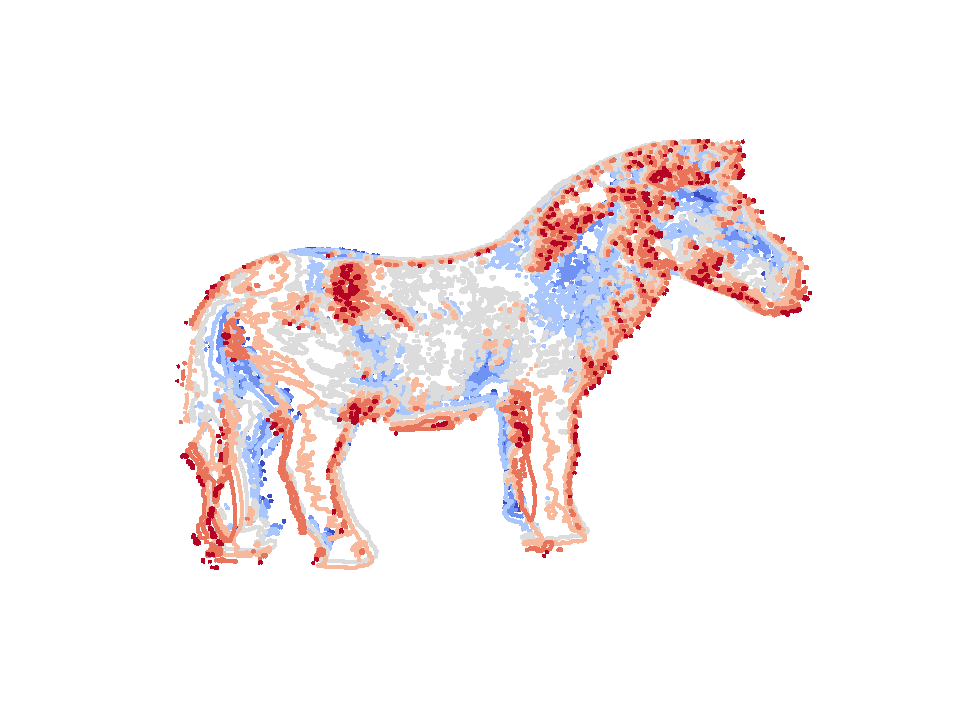
\includegraphics[scale=0.6]{informe/imagenes/supnivel/supNivelCaballoLucesPropias578N1.pdf} \\
}
{\centering
    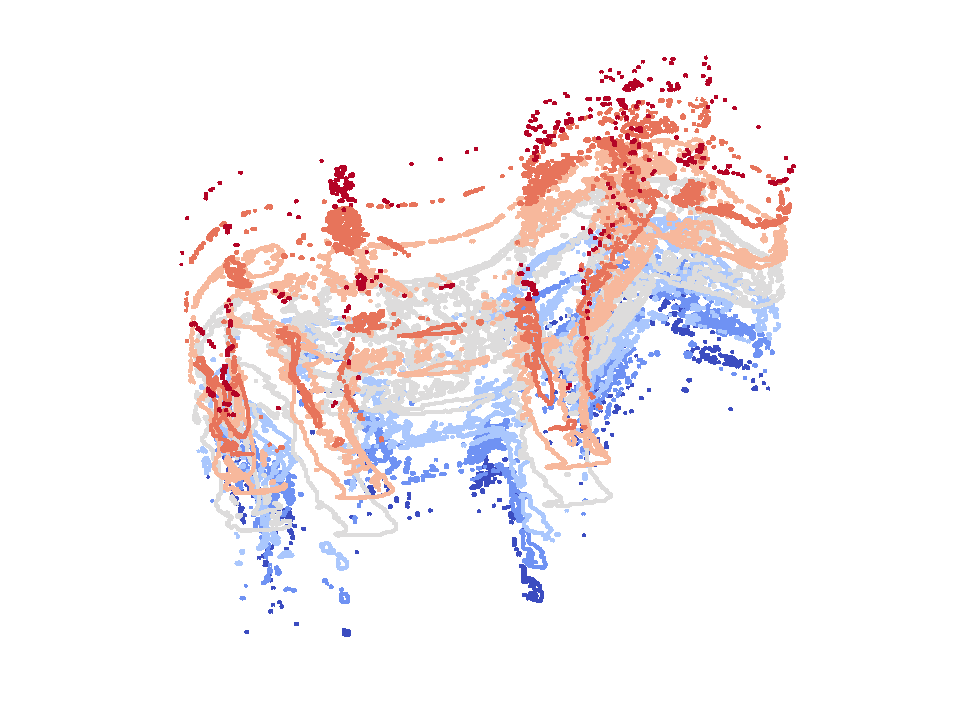
\includegraphics[scale=0.6]{informe/imagenes/supnivel/supNivelCaballoLucesPropias578N2.pdf} \\
}
{\centering
    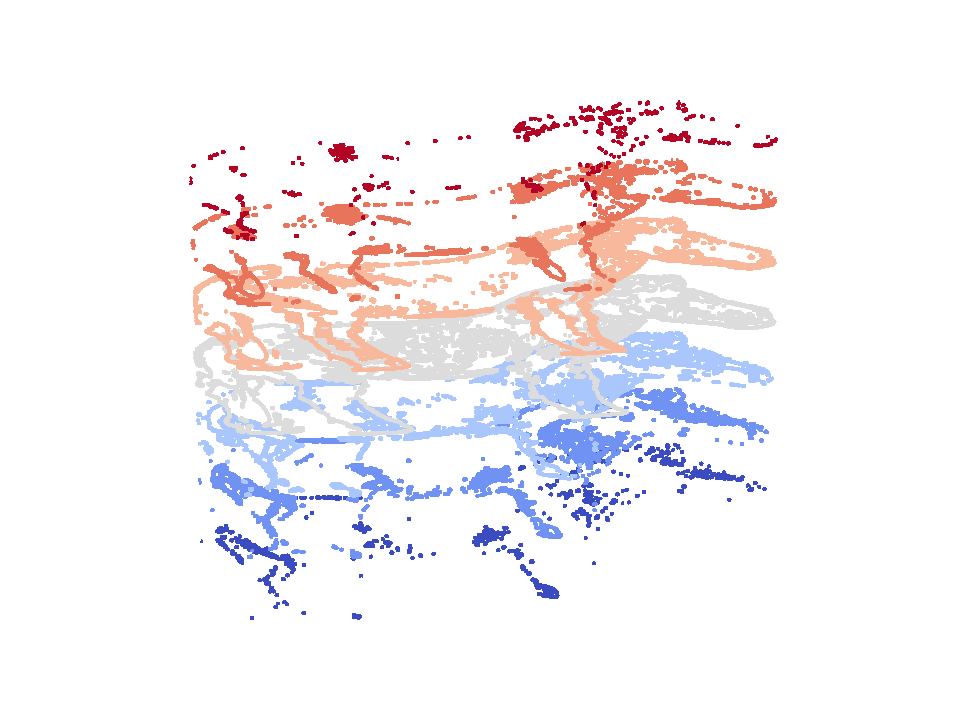
\includegraphics[scale=0.6]{informe/imagenes/supnivel/supNivelCaballoLucesPropias578N3.pdf} \\
}

{\centering
    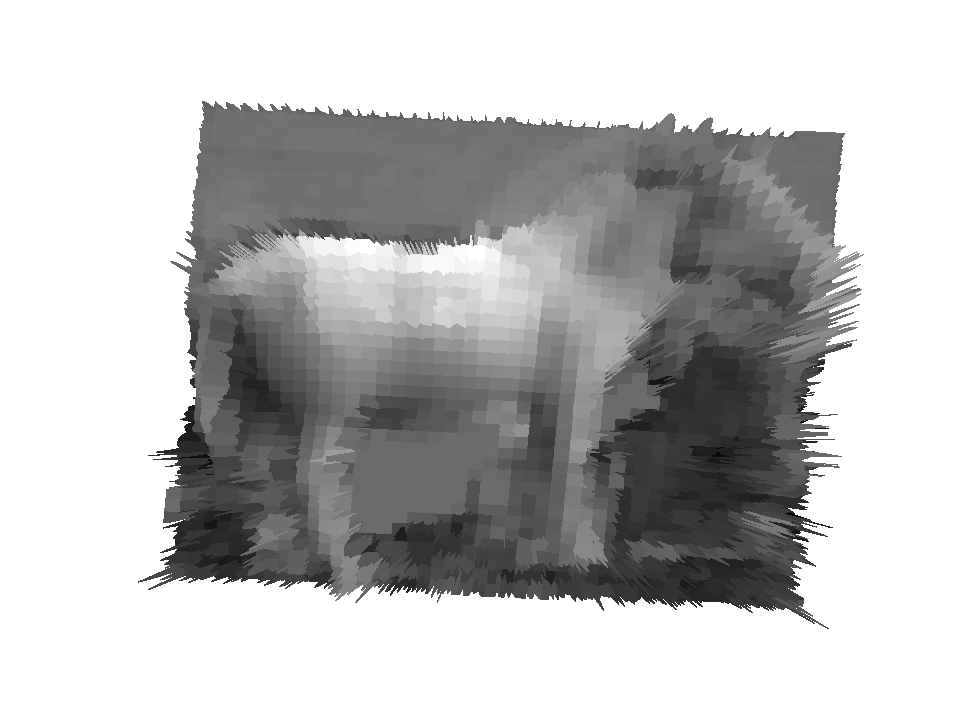
\includegraphics[scale=0.7]{informe/imagenes/profundidadesCaballoNormalescatedra.pdf} \\
}
